\section{Poisson Processes}
\label{sec:Poisson-Processes}

The Poisson process is the most widely used model for arrivals into a system because it is often a realistic representation of natural models and, since it exposes the Markovian property, it is analytically tractable.
It greatly models natural process where we observe aggregation of large number of independent entities \footnote{This is true thanks to the Limiting Theorem \cite{ross2014introduction}}.

The Poisson distribution is a discrete probability distribution that expresses the probability of a given number of events occurring in a fixed interval of time and/or space if these events occur with a known average rate and independently of the time since the last event. If inter-arrival times are Exponentially distributed, then the number of arrivals within a given time is Poisson distributed.

\begin{definition}[Poisson Distribution]
\label{def:Poisson-Distribution}
	A random variable $N(t)$ is Poisson distributed with rate\footnote{if $N(t) \sim Poisson(\lambda)$, $\lambda$ is called \textit{rate} because $\expected{N(t)}=\lambda t$.} $\lambda$ ($N(t) \sim Poisson(\lambda)$) if $N(t)$ has the following probability mass function:
	
	\begin{equation}
	\label{eqn:Poisson-PMF}
	f(k,t) = \frac{(\lambda t)^{k} e^{-\lambda t}}{k!}
	\end{equation}
\end{definition}

The p.d.f of $X \sim Poisson(\lambda)$ is shown in \Cref{fig:poisson-pdf}.

\begin{figure}[tp]
\label{fig:Poisson-PMF}	
	\centering
	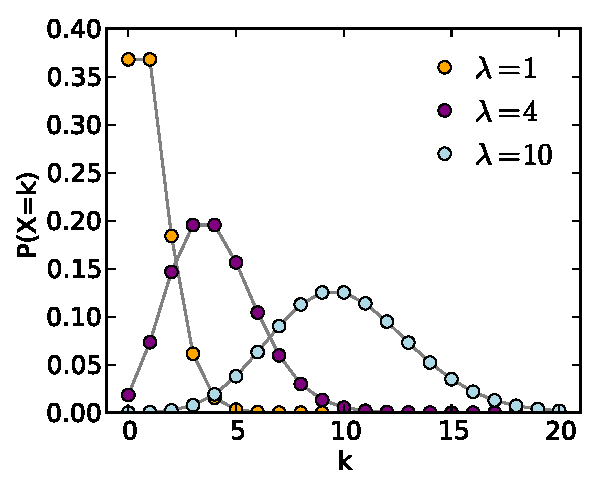
\includegraphics{fig/poisson-pdf}
	\caption{Poisson p.m.f.}
\end{figure}

From the \Cref{def:Poisson-Distribution} follows that the cumulative distribution function of $N(t) \sim Poisson(\lambda)$ is 

\begin{equation}
\label{eqn:Poisson-CDF}
F(k,t) = \sum_{x=0}^{t} f(k,x)
\end{equation}

The Poisson distribution has mean

\begin{equation}
\label{eqn:Poisson-Mean}
\expected{N(t)} = \lambda t
\end{equation}

and variance

\begin{equation}
\label{eqn:Poisson-Variance}
\variance{N(t)} = \lambda t
\end{equation}

\begin{definition}[Poisson Process]
\label{def:poisson-process-statistical}
	A Poisson process with rate $\lambda$ is a sequence of events such that
	(i) $N(0)=0$,
	(ii) it has independent increments,
	(iii) $\probability{N(s+t)-N(s) = n} \sim Poisson(\lambda t)$
\end{definition}

Notice that point (iii) in \Cref{def:poisson-process-statistical} implies stationary increments. 
Furthermore, the assumption of independent and stationary increments implies that, at any point in time, the process statistically restarts itself; that is, the process from any point onward is independent of all previously occurred (independent increments) and has the same distribution of the original process (stationary increments).

\begin{definition}[Poisson Process]
\label{def:poisson-process-practical}
	A Poisson process with rate $\lambda$ is a sequence of events such that
	(i) the interarrival times are Exponential r.v. with rate $\lambda$, and 
	(ii) $N(0)=0$.
\end{definition}

A Poisson process has stationary and independent increments.

Here are some useful properties of the Poisson distribution.

\begin{theorem}[Poisson Merging]
\label{thm:Poisson-Merging}	
	Given two independent Poisson process with rate $\lambda_{1}$ and $\lambda_{2}$, the merged process is a Poisson process with rate $(\lambda_{1} + \lambda_{2})$.
\end{theorem}

\begin{theorem}[Poisson Splitting]
\label{thm:Poisson-Splitting}	
	Given a Poisson process with rate $\lambda$, whose events are partitioned in class-A with probability $p$ and class-B with probability $(1-p)$, the class-A process is a Poisson process with rate $p \lambda$ and the class-B process is a Poisson process with rate $(1-p) \lambda$, and these processes are independent.
\end{theorem}

\begin{theorem}[Poisson Uniformity - Single Event]
\label{thm:Poisson-Uniformity-Single-Event}	
	Given that one event of a Poisson process has occurred by time $t$, that event is equally likely to have occurred anywhere in $[0,t]$. 
\end{theorem}

\begin{theorem}[Poisson Uniformity - Multiple Events]
\label{thm:Poisson-Uniformity-Multiple-Events}	
	If $k$ events of a Poisson process occur by time $t$, then the $k$ events are distributed independently and uniformly in $[0,t]$. 
\end{theorem}